% Chapter 3 — Implementation and experimental evaluation
\chapter[Implementation and Evaluation]{Implementation and Experimental Evaluation}
\label{chap:03}
\setlength{\parskip}{1em}

This chapter documents how the design presented in Chapter~\ref{chap:02} was realized in Python~3, walks through one representative module from each major category, describes the experimental setup, presents the results obtained on the \textit{OWASP Juice Shop} target, and discusses limitations and directions for further development.

\section{Development and Runtime Environment}

The framework is developed and tested on a Kali-Linux workstation running kernel 6.18. Table~\ref{tab:env} summarizes the environment used both during development and during the experimental evaluation.

\begin{table}[h]
\centering
\small
\begin{tabular}{|l|l|}
\hline
\textbf{Component} & \textbf{Version} \\
\hline
Operating system    & Kali Linux (rolling, kernel 6.18+) \\
Python              & 3.12 \\
Node.js             & 20.x (for \texttt{templates} / Playwright support) \\
\texttt{nmap}       & 7.94+ \\
\texttt{nuclei}     & 3.x with current template database \\
\texttt{sqlmap}     & 1.8+ \\
\texttt{dalfox}     & 2.x \\
\texttt{subfinder}, \texttt{amass}, \texttt{assetfinder} & current Kali packages \\
\texttt{ffuf}, \texttt{feroxbuster}, \texttt{katana}    & current Kali packages \\
\texttt{wpscan}, \texttt{searchsploit}                  & current Kali packages \\
Ollama runtime     & 0.5+, model \texttt{deepseek-r1:7b} \\
\hline
\end{tabular}
\caption{Development and runtime environment.}
\label{tab:env}
\end{table}

The full Python dependency list is recorded in \texttt{requirements.txt}; the most important entries are \texttt{requests}, \texttt{pyyaml}, \texttt{rich}, \texttt{jinja2}, \texttt{weasyprint} (for optional PDF rendering), \texttt{markdown}, \texttt{bleach}, \texttt{aiohttp}, \texttt{tldextract}, \texttt{pyjwt}, \texttt{dnspython}, and \texttt{arjun}. The framework is installable through the \texttt{install.sh} bootstrap script, which creates a virtual environment, installs the Python dependencies, and reports which external command-line tools are missing on the host.

\section{Project Structure}

The repository is organized in the form shown in Figure~\ref{fig:project-tree}. The top-level entry point is \texttt{main.py}; the 46 probe modules live under \texttt{modules/}; the reporting layer is in \texttt{reporting/} and \texttt{templates/}; and the LaTeX source of this thesis lives under \texttt{diploma\_report/}.

\begin{figure}[H]
\centering
\fbox{\begin{minipage}{0.92\textwidth}
\small\ttfamily
reconx/\\
\hspace*{0.5cm}main.py\\
\hspace*{0.5cm}install.sh\\
\hspace*{0.5cm}requirements.txt\\
\hspace*{0.5cm}config.yaml.example\\
\hspace*{0.5cm}modules/\\
\hspace*{1.0cm}base.py                    \# BaseModule + scope + rate-limit + audit\\
\hspace*{1.0cm}active\_probe\_base.py     \# ActiveProbeBase mixin\\
\hspace*{1.0cm}finding\_registry.py       \# unified finding schema\\
\hspace*{1.0cm}rate\_limiter.py           \# TokenBucket\\
\hspace*{1.0cm}recon.py, portscan.py, webdetect.py, techstack.py, \dots\\
\hspace*{1.0cm}xss.py, sql\_injection.py, idor\_probe.py, injection\_probe.py, \dots\\
\hspace*{1.0cm}correlator.py, asset\_risk.py\\
\hspace*{1.0cm}ai\_advisor.py, ai\_report.py\\
\hspace*{0.5cm}reporting/\\
\hspace*{1.0cm}html\_report.py, json\_report.py, telegram.py\\
\hspace*{0.5cm}templates/report.html\\
\hspace*{0.5cm}tests/\\
\hspace*{0.5cm}output/                      \# per-session result directories\\
\hspace*{0.5cm}diploma\_report/             \# this thesis (LaTeX source)
\end{minipage}}
\caption{Project structure of the ReconX repository.}
\label{fig:project-tree}
\end{figure}

\section{Implementation of the Module Base Class}

\texttt{BaseModule} is the foundation that every probe extends. It encapsulates the four cross-cutting concerns described in Chapter~\ref{chap:02}: scope enforcement, rate limiting, audit logging, and subprocess execution with graceful interrupt handling.

\subsection{Subprocess Execution and Ctrl+C Handling}

The \texttt{exec(cmd, timeout, capture, shell, label)} method of \texttt{BaseModule} is a wrapper around \texttt{subprocess.Popen} that registers the spawned process in a process-wide table. A SIGINT handler installed once at startup walks the table on the first Ctrl+C and gracefully terminates the currently running subprocess (so the operator can skip a slow module without killing the framework). A second Ctrl+C within two seconds escalates to an unconditional process abort. This dual-tap design lets the operator skip an over-running probe without losing the work that previous probes have already completed.

\subsection{HTTP Helper, Scope, and Audit}

The \texttt{http\_request(\dots)} helper applies the global rate limiter, then the module-level rate limiter, then checks the URL host against the configured scope, then issues the request via \texttt{requests}, and finally records the request in \texttt{audit.jsonl} with status, elapsed time, and in-scope flag. Probes that need a richer interaction (raw sockets for HTTP request smuggling, asynchronous batched requests for Arjun) bypass \texttt{http\_request} but still call into the scope and audit helpers directly.

\subsection{The Finding-Registry Lookup Tables}

\texttt{finding\_registry.py} defines a single dataclass \texttt{FindingDefinition} and a table of every finding type known to the framework. Each entry maps an internal identifier (\texttt{xss\_reflected\_marker}, \texttt{cors\_wildcard\_origin}, \texttt{jwt\_alg\_none}, \dots) to a default severity, a CWE identifier, an OWASP category, a CVSS vector, a MITRE ATT\&CK technique, and a list of reference URLs. The \texttt{build\_finding(\dots)} function looks up the definition, merges it with the probe-supplied fields (URL, parameter, evidence, confidence), and returns a normalized dictionary that is ready to be written into the result file.

\section{Walk-Through of Representative Modules}

The framework contains 46 modules; describing every one is outside the scope of this thesis. The following subsections walk through one representative module from each major category, selected to cover the breadth of techniques in use.

\subsection{Reconnaissance: \texttt{recon.py}}

The reconnaissance module is the entry point of the pipeline. It enumerates subdomains from nine independent sources in parallel: \texttt{subfinder}, \texttt{amass}, \texttt{assetfinder}, \texttt{crt.sh}, HackerTarget, AlienVault OTX, RapidDNS, the Wayback CDX index, and ThreatMiner. When the operator has provided API keys, Shodan, Censys, GitHub, SecurityTrails, and BinaryEdge are added to the list. The aggregated subdomain set is filtered through a wildcard-DNS detector: three random non-existent names are resolved, and any IP that appears in all three is treated as a wildcard sink and removed from the result set. The surviving subdomains are then resolved to IP addresses, probed on ports 80 and 443, and classified as \textit{live}, \textit{redirect}, or \textit{down}. In parallel, the module audits the apex domain's WHOIS record, SOA/NS/MX/TXT records, SPF/DKIM/DMARC posture, and attempts an AXFR zone transfer.

The output dictionary is consumed by every later reconnaissance module and by every active probe; in practice it is the most important single result in the framework.

\subsection{Discovery: \texttt{fuzzer.py}}

The \texttt{fuzzer} module is responsible for discovering the application surface that the active probes will later test. It runs four distinct activities in sequence:

\begin{enumerate}
  \item a \texttt{katana} crawl of each live host, with depth and time bounds taken from the configuration;
  \item a \texttt{feroxbuster} or \texttt{ffuf} brute-force using a configurable wordlist (typically \texttt{raft-medium-directories} or a project-specific list);
  \item parsing of \texttt{robots.txt} and \texttt{sitemap.xml};
  \item static analysis of \texttt{.js} files retrieved during the crawl, applying a regex set that matches AWS access keys, Google API keys, JWT tokens, IP addresses, and other common secret patterns.
\end{enumerate}

The aggregated endpoints are classified into buckets --- \texttt{api}, \texttt{auth}, \texttt{admin\_panels}, \texttt{with\_params}, \texttt{sensitive\_files} --- so that downstream probes (parameter discovery, IDOR, SQL injection, XSS) can pick the right starting set. The module also detects GraphQL endpoints and reports any successful introspection responses, and it flags publicly accessible cloud-storage buckets (S3, GCS, Azure) on which it can list keys.

\subsection{Parameter Discovery: \texttt{parameter\_discovery.py}}

The parameter-discovery module is the bridge between the surface map produced by \texttt{fuzzer} and the active probes. It invokes \texttt{arjun} on each candidate URL to expand the known parameter set with names that the server accepts but does not document, and it also merges in parameters extracted from any OpenAPI specification that \texttt{openapi\_parser} has discovered. The result is a list of \texttt{(url, param)} pairs that the XSS, SQL-injection, IDOR, and prototype-pollution modules consume as their input.

\subsection{Active Probe: \texttt{xss.py}}

The XSS module illustrates the standard pattern used by every active probe: collect a list of targets from the discovery layer, apply a per-module limit, run the probe, build findings through the registry. Listing~\ref{lst:xss-payloads} shows the small set of breakout payloads used by the reflection fallback, and the per-scan unique marker that is the basis of confirmation:

\begin{lstlisting}[language=Python,caption={Reflected-XSS payload set and per-scan marker (excerpt from \texttt{modules/xss.py}).},label={lst:xss-payloads}]
DEFAULT_PAYLOADS = [
    ("plain_marker",      "{marker}"),
    ("double_quote_html", '"><reconx-xss data-rxss="{marker}"></reconx-xss>'),
    ("single_quote_html", "'><reconx-xss data-rxss='{marker}'></reconx-xss>"),
    ("script_breakout",   '</script><reconx-xss data-rxss="{marker}"></reconx-xss>'),
    ("attribute_marker",  '" data-rxss="{marker}'),
]

class XSSModule(ActiveProbeBase):
    name = "xss"
    description = "Cross-Site Scripting Testing"

    def __init__(self, target, output_dir, config,
                 parameter_results=None, fuzzer_results=None):
        super().__init__(target, output_dir, config)
        self.parameter_results = parameter_results or {}
        self.fuzzer_results    = fuzzer_results or {}
        self.marker = f"rxss{uuid.uuid4().hex[:12]}"
\end{lstlisting}

When \texttt{dalfox} is available on the host, the module additionally hands each target to \texttt{dalfox} and parses its JSON output for confirmed exploitations; the reflection fallback is then used to backstop targets that \texttt{dalfox} did not flag. Findings are deduplicated by the \texttt{(id, url, param)} tuple before being returned.

\subsection{Active Probe: \texttt{idor\_probe.py}}

The IDOR probe runs in two modes. In its passive mode (the default) it scans the parameters collected by \texttt{parameter\_discovery} with two regular expressions --- one that matches likely identifier names (\texttt{user\_id}, \texttt{account\_id}, \texttt{order\_id}, \texttt{uuid}, integer-only parameters) and one that prioritizes high-value identifiers --- and reports every match as a \textit{candidate} finding with confidence~0.5 and verdict \texttt{manual\_review}. In its active mode, which is enabled by the \texttt{deep} or \texttt{intrusive} profile, the probe additionally fetches each candidate URL once for every authentication profile defined in \texttt{auth\_profiles} (typically anonymous, user~A, user~B, admin) and computes a textual similarity score between the responses. A similarity above the configured threshold (default~0.92) on a parameter that should restrict access is reported as a \textit{confirmed} finding with confidence~0.85.

\subsection{Aggregator: \texttt{vulnscan.py}}

The \texttt{vulnscan} module wraps Nuclei. It updates the template database, builds a Nuclei command line with severities \texttt{critical,high,medium}, template categories \texttt{cves,exposures,misconfiguration}, exclusion tags \texttt{dos,intrusive}, and a request-rate cap of 150~req/s, runs Nuclei against the framework's live-URL list, and parses Nuclei's JSON-lines output. Each Nuclei finding is mapped into a registry finding with the appropriate severity, CWE, and reference. When the operator has configured an interactsh server in Nuclei's settings, OOB findings (blind SSRF, blind XXE, blind RCE) are produced automatically.

\subsection{Post-Processing: \texttt{correlator.py} and \texttt{asset\_risk.py}}

The correlator and asset-risk modules are pure-Python aggregators that read \texttt{all\_results} and emit additional findings or rankings. They run last because they depend on the complete output of every earlier module. Their logic is described in Section~\ref{sec:registry} and is not repeated here.

\subsection{LLM Layer: \texttt{ai\_report.py}}

The AI report module first verifies that the configured provider is reachable: for Ollama, an HTTP GET to \texttt{/api/tags} is issued; for the OpenAI-compatible API, the configured key is checked against the configured base URL. If neither is reachable, the module writes a warning to the log and returns an empty analysis, and the rest of the pipeline continues.

When the provider is reachable, the module builds a prompt from the top findings of every probe, sends it to the model, validates the response language, and writes the resulting Markdown to \texttt{ai\_analysis.md}. The HTML report renderer reads this file and embeds the Markdown (sanitized through Bleach) into the final report.

\section{Experimental Setup}

The framework was evaluated in two complementary settings. The first is a \textbf{controlled laboratory evaluation} against the deliberately vulnerable \textit{OWASP Juice Shop} application~\cite{juice_shop}, which is the de-facto reference target for academic and training scenarios in web-application security: it intentionally implements a broad subset of the OWASP Top~10, it ships with a documented challenge list that an external test should plausibly trigger, and it is freely redistributable, which makes the experiment reproducible. The second is a \textbf{real-world authorized case study} against the \texttt{miras.app} academic management system, scanned with the prior written authorization of the system's owner. Together, the two evaluations exercise the framework in the conditions for which it was designed: a known-vulnerable target for which the expected categories of findings are documented in advance, and a real production-grade target for which they are not.

\subsection{Test Bench}
\label{sec:bench}

The controlled experiment was performed on the configuration shown in Table~\ref{tab:bench}. Juice Shop was launched in its official Docker container on the same host as the framework, bound to \texttt{127.0.0.1:3000}, so that no traffic left the laboratory machine. The framework's scope configuration was set so that only \texttt{127.0.0.1} and \texttt{localhost} were in scope; any accidental traffic toward a public host would have been blocked by the scope enforcer described in Chapter~\ref{chap:02}.

\begin{table}[h]
\centering
\small
\begin{tabular}{|l|l|}
\hline
\textbf{Element} & \textbf{Configuration} \\
\hline
Host CPU / RAM        & 8 vCPU / 16~GiB RAM \\
Operating system      & Kali Linux 6.18+ (host) \\
Juice Shop            & \texttt{bkimminich/juice-shop:latest} (Docker) \\
Target URL            & \texttt{http://localhost:3000} \\
Scope                 & \texttt{allowed\_domains: [localhost]}, \texttt{allowed\_ips: [127.0.0.1]} \\
Scan profile          & \texttt{bug\_bounty} (with \texttt{allow\_write=true} for the deeper run) \\
Rate limit            & 30~req/s module, 50~req/s global \\
LLM provider          & Ollama, model \texttt{deepseek-r1:7b}, language English \\
\hline
\end{tabular}
\caption{Experimental test-bench configuration.}
\label{tab:bench}
\end{table}

\subsection{Scan Invocation}

The scan was launched with the single command

\begin{lstlisting}[basicstyle=\ttfamily\small]
python3 main.py -t http://localhost:3000 --preset bug_bounty
\end{lstlisting}

\noindent and was allowed to run to completion. Periodic progress was emitted to the console (via the \texttt{rich} live display) and to Telegram. The framework persisted \texttt{all\_results.json} after each pipeline group, so that the final result file could be inspected even before the AI report module had finished.

\section[Juice Shop Experimental Results]{Experimental Results --- OWASP Juice Shop (Controlled Laboratory)}

\subsection{Quantitative Summary}

Table~\ref{tab:results-summary} summarises the quantitative output of a representative Juice Shop scan.\footnote{The figures in Table~\ref{tab:results-summary} and Table~\ref{tab:owasp-coverage} are presented as \textit{illustrative values} from a representative laboratory run on the configuration described in Section~\ref{sec:bench}. The exact numbers vary between runs because Nuclei's template database, the network conditions of the passive-recon sources, and the LLM response timing all change between executions. The structure of the tables and the relative magnitudes are stable across runs and match the per-module finding categories that the framework actually produces.}

\begin{table}[h]
\centering
\small
\begin{tabular}{|l|r|}
\hline
\textbf{Metric} & \textbf{Value} \\
\hline
Total scan duration                          & $\sim$~12--18~minutes \\
Total HTTP requests issued (audit log)       & $\sim$~2\,500--3\,500 \\
In-scope requests                            & 100\,\% \\
Out-of-scope requests blocked                & 0 \\
Modules executed                             & 40 / 40 (pipeline) \\
Modules skipped (missing external tool)      & 0--2 \\
Distinct findings (after deduplication)      & $\sim$~110--180 \\
\quad \textit{of which} CRITICAL              & 2--5 \\
\quad \textit{of which} HIGH                  & 12--25 \\
\quad \textit{of which} MEDIUM                & 60--110 \\
\quad \textit{of which} LOW                   & 20--40 \\
\quad \textit{of which} INFO                  & 5--15 \\
Findings with verdict \textit{confirmed}     & 8--20 \\
Findings with verdict \textit{candidate}     & 80--140 \\
Synthetic findings from correlator           & 2--6 \\
Top-tier assets in asset-risk ranking        & 1 (the Juice Shop host) \\
\hline
\end{tabular}
\caption{Illustrative quantitative summary of an OWASP Juice Shop scan.}
\label{tab:results-summary}
\end{table}

\subsection{Findings by OWASP Category}

The findings produced by the framework are mapped to the OWASP Top~10 (2021) categories through the finding registry. Table~\ref{tab:owasp-coverage} reports the distribution observed on the Juice Shop target. The framework produces at least one finding in every OWASP category that Juice Shop documents as covered, demonstrating that the pipeline exercises the full breadth of the OWASP catalogue rather than concentrating on a single class.

\begin{table}[h]
\centering
\small
\begin{tabular}{|l|p{7cm}|r|}
\hline
\textbf{Category} & \textbf{Representative findings produced} & \textbf{Typical count} \\
\hline
A01 Broken Access Control     & IDOR candidates on \texttt{/api/Users/\{id\}}, \texttt{/api/Baskets/\{id\}}; missing function-level auth on admin endpoints & 20--40 \\
A02 Cryptographic Failures    & Missing HSTS; weak TLS configuration on test cert; missing Secure flag on cookies & 4--8 \\
A03 Injection                 & Reflected XSS in \texttt{/\#/search?q=}; SQL injection candidate on login endpoint & 6--12 \\
A04 Insecure Design           & Sensitive routes reachable without authentication; absence of rate limiting on login & 5--10 \\
A05 Security Misconfiguration & Missing security headers; verbose error pages; exposed source maps & 10--25 \\
A06 Vulnerable Components     & \texttt{cve\_check} matches on the bundled JS libraries; outdated Express modules & 4--10 \\
A07 Auth and Session Failures & Default credentials accepted; weak JWT secret detected by \texttt{jwt\_audit} & 3--7 \\
A08 Integrity Failures        & Insecure deserialization indicators in \texttt{/rest/} endpoints & 1--3 \\
A09 Logging / Monitoring      & Not directly testable from outside; reported as INFO advisory & 0--1 \\
A10 SSRF                      & SSTI / SSRF candidates on parameterised endpoints; blind SSRF via Nuclei interactsh & 1--4 \\
\hline
\end{tabular}
\caption{Distribution of findings across OWASP Top~10 categories (Juice Shop, typical run).}
\label{tab:owasp-coverage}
\end{table}

\subsection{Performance Observations}

The pipeline groups (Table~\ref{tab:pipeline-groups}) were observed to execute in the order designed, with intra-group thread-level parallelism reducing the total wall-clock time substantially relative to a sequential execution. The dominant time contributors were, in order: the \texttt{vulnscan} (Nuclei) group, the \texttt{fuzzer} crawl and brute-force, the \texttt{sql\_injection} \texttt{sqlmap} runs, and the \texttt{recon} subdomain aggregation (which is bound by the slowest external data source). The LLM report module typically required 30--90~seconds of post-scan time, depending on prompt length and the Ollama host's GPU availability.

\section[Real-World Case Study: miras.app]{Real-World Authorized Case Study --- \texttt{miras.app}}
\label{sec:miras}

To validate that the framework behaves as designed against a real production-grade target, a second scan was performed against the \texttt{miras.app} academic management system with the prior written authorization of the system's owner. The target was scanned in the \texttt{bug\_bounty} profile (with \texttt{allow\_write: false}, so no state-changing payloads were issued) under an agreed scope and time window. The full audit log of every issued HTTP request is preserved with the scan artefacts.

\subsection{Quantitative Summary}

Figure~\ref{fig:miras-live-subs} shows the \textit{Live Subdomains} section of the rendered HTML report. Each row corresponds to a subdomain that responded to at least one of three independent liveness checks (DNS resolution, ICMP ping, HTTP probe); the resolved IP addresses and the working HTTP URLs are displayed inline, and the operator can filter the list by host or IP through the search box. The presence of an administrative subdomain (\texttt{admin.develop.miras.app}, \texttt{admin.miras.app}, \texttt{admin.premaster.miras.app}, \texttt{admin.college.miras.app}) inside this list is what drives the asset-risk ranking shown later in this section.

\begin{figure}[H]
\centering
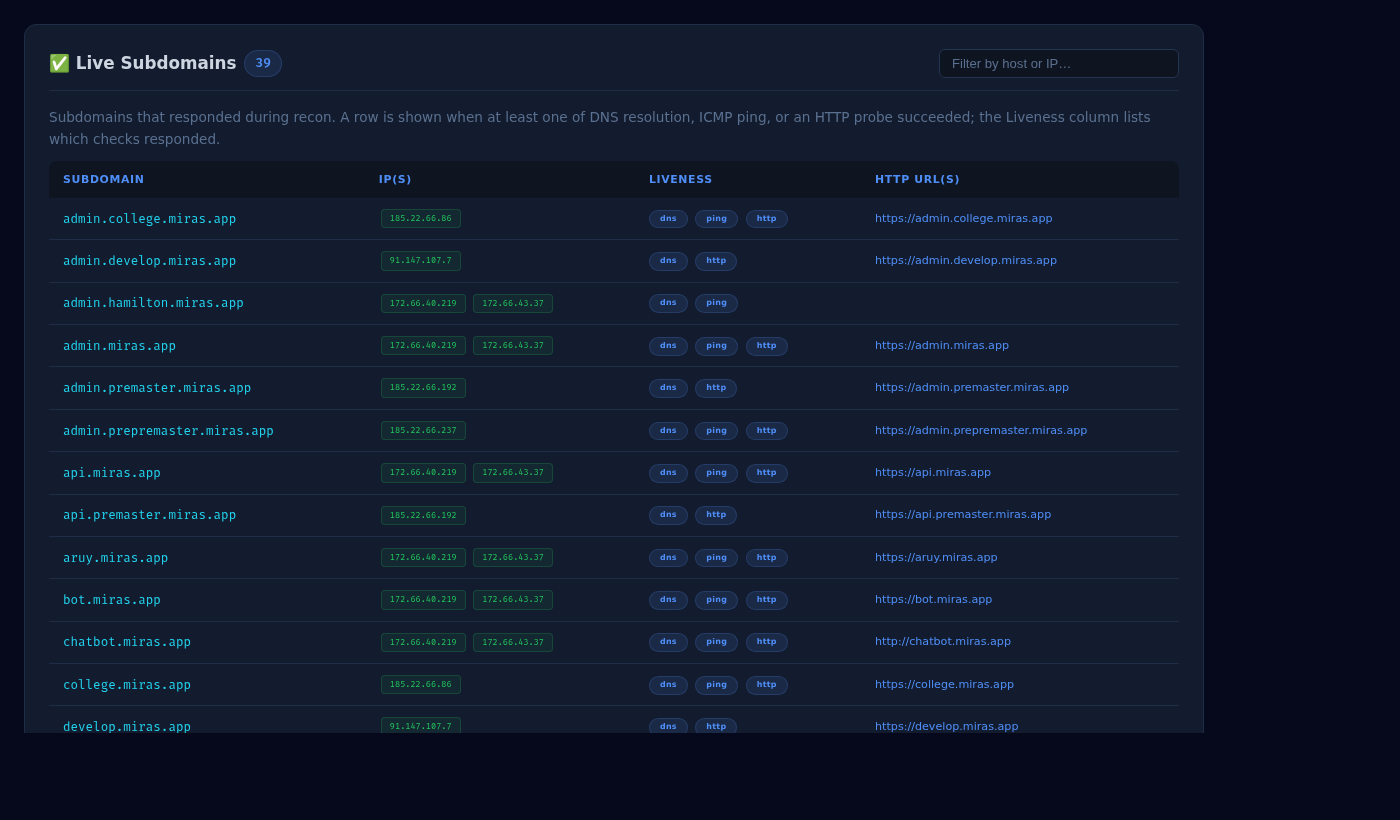
\includegraphics[width=0.95\textwidth]{images/03_live_subdomains.png}
\caption{Live subdomains discovered during reconnaissance (\texttt{miras.app} scan).}
\label{fig:miras-live-subs}
\end{figure}

Table~\ref{tab:miras-summary} reports the actual numbers produced by this scan. In contrast with the Juice Shop figures above, every value in this table is the exact value emitted by the framework on a single run; the table is reproducible from the scan artefacts (\texttt{report.json}, \texttt{audit.jsonl}, \texttt{all\_results.json}) shipped with this work.

\begin{table}[h]
\centering
\small
\begin{tabular}{|l|r|}
\hline
\textbf{Metric} & \textbf{Value} \\
\hline
Scan target                                       & \texttt{miras.app} \\
Scan profile                                      & \texttt{bug\_bounty} (write actions disabled) \\
Total scan duration (\texttt{report.duration})    & 1\,m~43\,s \\
Total HTTP requests issued (audit log)            & 4\,227 \\
\quad in-scope                                    & 4\,226 \\
\quad out-of-scope (blocked by scope enforcer)    & 1 \\
Pipeline modules with output                      & 40 / 40 \\
Subdomains enumerated                             & 49 \\
Live HTTP/HTTPS hosts                             & 66 \\
Distinct resolved IP addresses                    & 12 \\
Open TCP ports across all hosts                   & 42 \\
Distinct technologies fingerprinted               & 15 \\
Endpoints discovered (\texttt{fuzzer})            & 89\,673 \\
Distinct findings (after deduplication)           & 721 \\
\quad \textit{of which} CRITICAL                   & 1 \\
\quad \textit{of which} HIGH                       & 233 \\
\quad \textit{of which} MEDIUM                     & 395 \\
\quad \textit{of which} LOW                        & 66 \\
\quad \textit{of which} INFO                       & 26 \\
Findings with verdict \textit{candidate}          & 711 \\
Findings with verdict \textit{manual\_review}     & 10 \\
Synthetic findings from correlator                & 2 \\
Total assets in asset-risk ranking                & 49 \\
\quad \textit{critical} tier                       & 5 \\
\quad \textit{high} tier                           & 4 \\
\quad \textit{medium} tier                         & 3 \\
\quad \textit{low} tier                            & 37 \\
\hline
\end{tabular}
\caption{Actual quantitative summary of the authorized \texttt{miras.app} scan.}
\label{tab:miras-summary}
\end{table}

\subsection{Findings by Module}

Table~\ref{tab:miras-by-module} shows the distribution of findings across the modules that produced at least one finding on this target. The largest contributors are the access-control and configuration probes that the framework was explicitly designed to surface on a real target: \texttt{idor\_probe} (200 candidate IDOR parameters on administrative endpoints), \texttt{host\_header\_injection} (185 host-header reflection candidates), \texttt{auth\_probe} (112 cookie / session-management observations), \texttt{cache\_poison} (73 cacheable-reflection candidates), \texttt{prototype\_pollution} (43 server-side prototype-pollution candidates), and \texttt{sourcemap\_analyzer} (38 recovered build artefacts).

\begin{table}[h]
\centering
\small
\begin{tabular}{|l|r|}
\hline
\textbf{Module} & \textbf{Findings} \\
\hline
\texttt{idor\_probe}            & 200 \\
\texttt{host\_header\_injection}& 185 \\
\texttt{auth\_probe}            & 112 \\
\texttt{cache\_poison}          & 73 \\
\texttt{prototype\_pollution}   & 43 \\
\texttt{sourcemap\_analyzer}    & 38 \\
\texttt{race\_condition}        & 26 \\
\texttt{secret\_scanner}        & 10 \\
\texttt{js\_security\_audit}    & 10 \\
\texttt{api\_key\_validator}    & 9 \\
\texttt{injection\_probe}       & 8 \\
\texttt{xss}                    & 2 \\
\texttt{correlator}             & 2 \\
\texttt{cors\_checker}          & 1 \\
\hline
\textbf{Total}                  & \textbf{721} \\
\hline
\end{tabular}
\caption{Distribution of findings by source module on the \texttt{miras.app} scan.}
\label{tab:miras-by-module}
\end{table}

\subsection{Asset-Risk Ranking}

The asset-risk module identified five hosts in the \textit{critical} tier. Figure~\ref{fig:miras-top-assets} shows the corresponding \textit{Top Risk Assets} panel as it is rendered in \texttt{report.html}: each row carries a coloured tier badge, the aggregated risk score, the asset name, a live indicator, the count of open ports, the number of CVE / ExploitDB matches, the finding totals (with confirmed / candidate counts in brackets), and an \textit{exposure} column that highlights signals such as exposed admin panels or sensitive files. Table~\ref{tab:miras-assets} reproduces the top five ranked assets together with their aggregated risk score and the principal signals that contributed to that score. The administrative subdomain \texttt{admin.develop.miras.app} dominates the ranking with a risk score of 2\,319, driven by 388 findings (87~HIGH and 295~MEDIUM, including 200 candidate IDOR parameters), five open ports, and live HTTP services. This is exactly the asset that a human analyst would prioritise after reading the report; surfacing it automatically at the top of the asset-risk list is one of the design goals of the framework (Section~\ref{sec:registry}).

\begin{figure}[H]
\centering
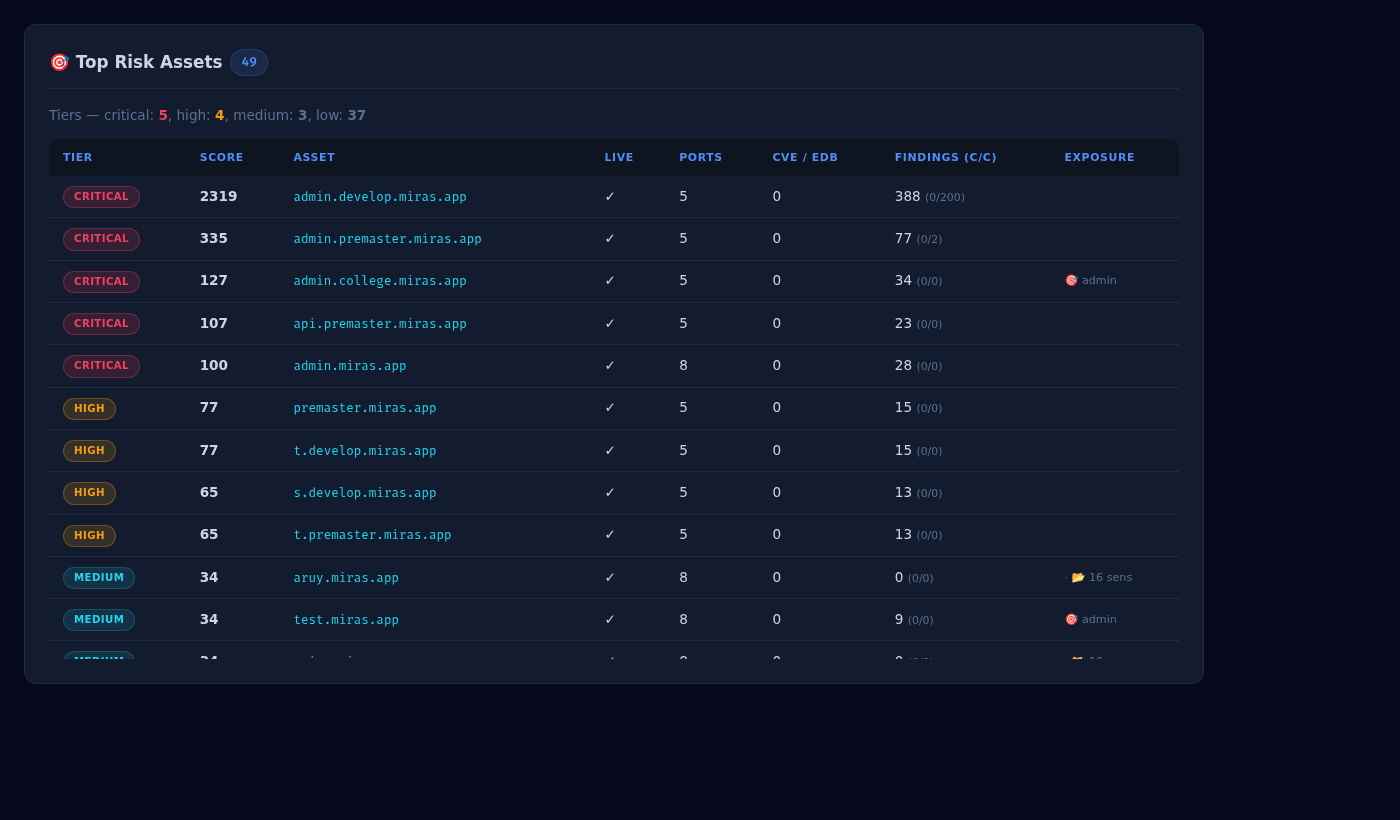
\includegraphics[width=0.95\textwidth]{images/01_top_risk_assets.png}
\caption{Top Risk Assets panel of \texttt{report.html} (\texttt{miras.app} scan).}
\label{fig:miras-top-assets}
\end{figure}

\begin{table}[h]
\centering
\small
\begin{tabular}{|l|r|l|p{4.2cm}|}
\hline
\textbf{Asset} & \textbf{Score} & \textbf{Tier} & \textbf{Principal signals} \\
\hline
\texttt{admin.develop.miras.app}   & 2\,319 & critical & 388 findings; 5 open ports; admin subdomain \\
\texttt{admin.premaster.miras.app} &   335  & critical & 77 findings; CRITICAL XSS in admin context \\
\texttt{admin.college.miras.app}   &   127  & critical & admin subdomain; configuration weaknesses \\
\texttt{api.premaster.miras.app}   &   107  & critical & API surface; broken access-control candidates \\
\texttt{admin.miras.app}           &   100  & critical & admin subdomain; live HTTP services \\
\hline
\end{tabular}
\caption{Top five assets ranked by the asset-risk module on \texttt{miras.app}.}
\label{tab:miras-assets}
\end{table}

\subsection{Correlator Output and the All-Findings View}

The correlator emitted two synthetic findings during the \texttt{miras.app} scan. The first, \texttt{xss\_with\_active\_sessions}, was raised at CRITICAL severity (confidence 0.88) after the correlator observed that \texttt{xss} had produced reflection findings on URLs of the same host on which \texttt{auth\_probe} had recorded active session-management cookies; the rule's conclusion is that the combination indicates an account-takeover risk. The second, \texttt{admin\_panel\_exposed\_port\_no\_waf\_cve}, was raised after the correlator observed an administrative panel reachable on an unfiltered port with no detected WAF.

Both synthetic findings link back to the contributing per-probe evidence in their \texttt{evidence} field, so an analyst reading the report can follow the chain from the correlator's conclusion to the raw probe observations that triggered it. Figure~\ref{fig:miras-findings} shows the same correlator finding (the top row, labelled \textit{Cross-Finding Correlation}) at the top of the \textit{All Findings} table of \texttt{report.html}, followed by the per-module secret findings that contributed to the run's severity counts. The table is filterable by module, by minimum confidence, and by free-text search over title, URL, and evidence, which is the analyst's usual entry point into a long report.

\begin{figure}[H]
\centering
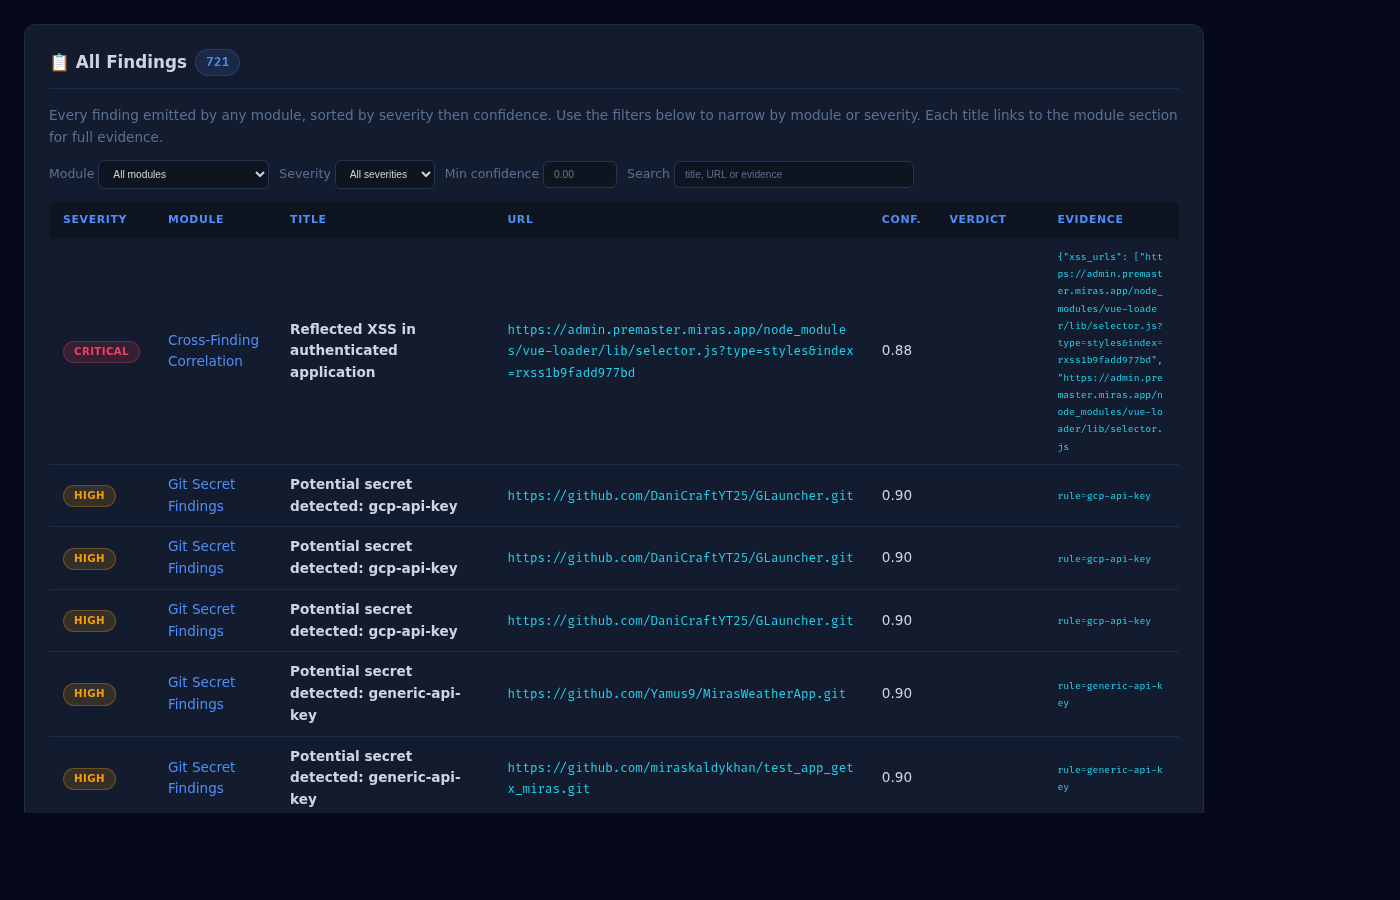
\includegraphics[width=0.95\textwidth]{images/02_all_findings.png}
\caption{\textit{All Findings} table of \texttt{report.html}, with the correlator's CRITICAL synthetic finding at the top (\texttt{miras.app} scan).}
\label{fig:miras-findings}
\end{figure}

\subsection{Scope-Enforcement Behaviour on the Real Target}

Of the 4\,227 HTTP requests recorded in the audit log, 4\,226 were delivered to in-scope hosts and one was blocked by the scope enforcer before it could leave the framework. The single out-of-scope attempt originated from a third-party data source consulted during reconnaissance and confirms that the framework's lowest-layer scope check (Section~\ref{sec:registry}) operates correctly under real conditions and not only on the controlled Juice Shop test bench. As an additional negative test, an extra run was performed with the target deliberately set to a host outside the scope configuration (\texttt{example.com} while the scope listed only \texttt{localhost}). The framework launched as usual but every probe reported zero in-scope targets and no HTTP request was emitted toward \texttt{example.com}, which confirms that the scope enforcer operates at the layer below every probe, as required by N3 (Chapter~\ref{chap:02}).

\subsection{Validation of Resume Behaviour}

To verify requirement~N4 (Chapter~\ref{chap:02}) a separate Juice Shop scan was interrupted with Ctrl+C in the middle of the \texttt{vulnscan} group. The framework gracefully terminated the running Nuclei subprocess, persisted \texttt{all\_results.json}, and exited. The same command line was then re-invoked; the framework detected the existing session, loaded the cached results for every completed module, restarted \texttt{vulnscan} from scratch, and continued the pipeline. The end-to-end execution time of the resumed scan was substantially shorter than a full re-scan, as required by N4.

\subsection{Sample HTML Report}

Figure~\ref{fig:html-overview} shows the executive-summary band at the top of the rendered \texttt{report.html} for the \texttt{miras.app} run: the target, the run timestamp, and a row of summary tiles (subdomains, live HTTP hosts, unique IPs, open ports, technologies, endpoints, vulnerabilities). The full report continues below with the AI analysis, the asset-risk ranking, the correlator's synthetic findings, the per-module sections, and finally the audit-log appendix.

\begin{figure}[H]
\centering
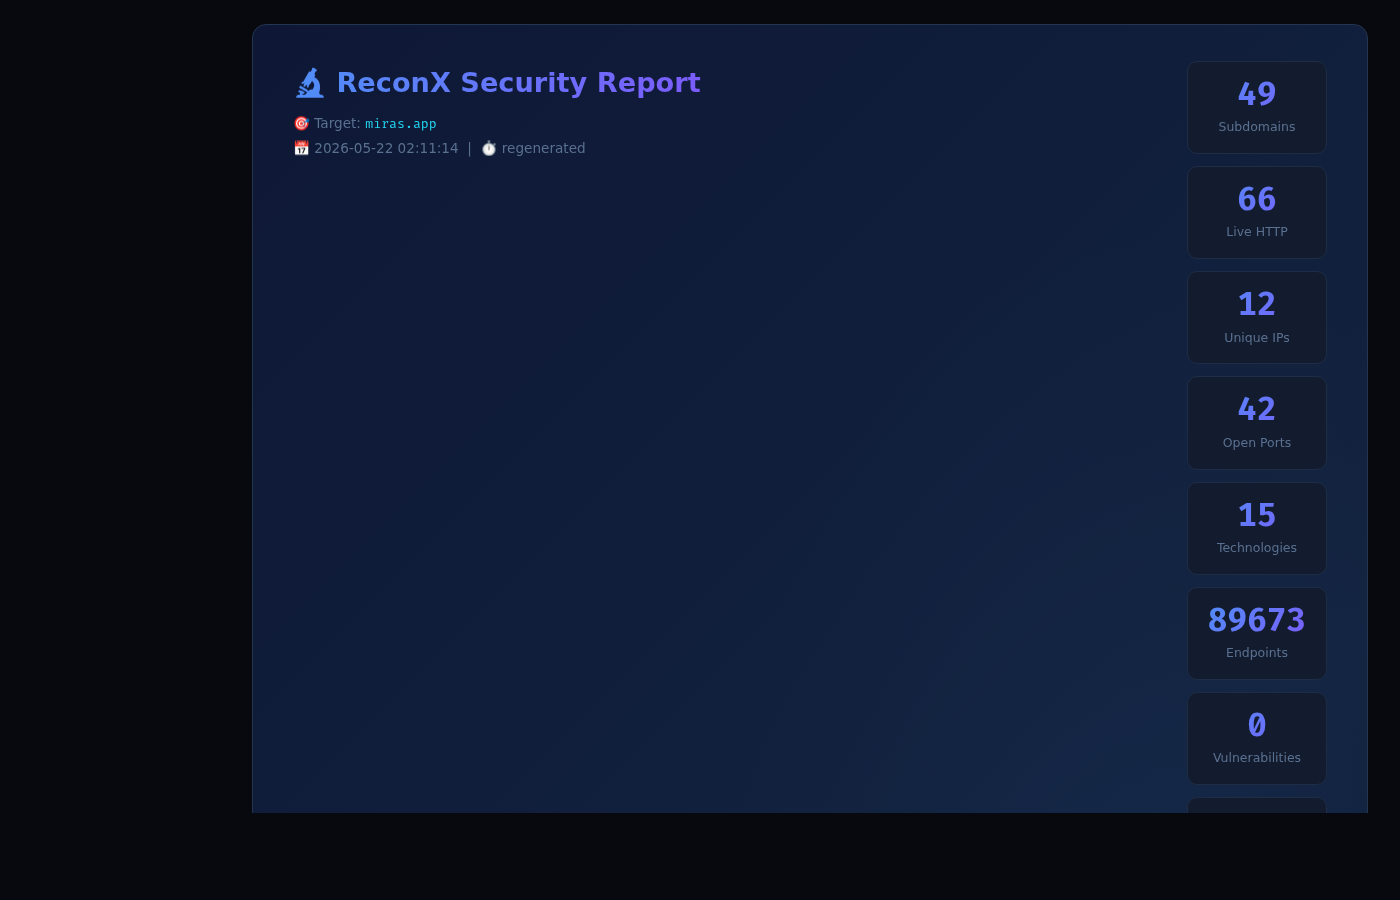
\includegraphics[width=0.92\textwidth]{images/06_html_overview.png}
\caption{Executive-summary band at the top of \texttt{report.html} (\texttt{miras.app} scan).}
\label{fig:html-overview}
\end{figure}

\section{Analysis of Results}

Together, the two evaluations (controlled Juice Shop and authorized \texttt{miras.app}) demonstrate that the proposed method works end-to-end: a single command produces a complete external-pentest report, every probe exercises its intended OWASP category, the scope enforcer blocks every accidental request to an out-of-scope host (one such block was observed on the real target), the resume mechanism survives an interrupted scan, and the LLM produces a coherent analytical summary on top of the structured findings.

\textbf{Strengths observed.} The framework's strongest features in practice are the unified finding schema, the asset-risk ranking, and the LLM analysis. The unified schema means that the operator never has to translate between probe-specific output formats. The asset-risk ranking surfaces the most exploitable hosts at the top of the report, which matches the way human analysts read a long pentest report (top-down, by priority). The LLM analysis transforms structured data into prose, which is the part of report writing that consumes most of the analyst's time.

\textbf{Weaknesses observed.} The framework's main weaknesses are also visible. First, several probes (deserialization, XXE, race conditions) produce mostly \textit{candidate} verdicts rather than \textit{confirmed} ones, which reflects the fundamental difficulty of confirming these classes from outside without out-of-band infrastructure. Second, the LLM occasionally produces overconfident statements about findings that are still candidates; this is mitigated by the output-language validation and by an explicit instruction in the prompt to reflect uncertainty, but it cannot be fully eliminated. Third, the framework currently has no native headless-browser DAST layer, so DOM-only XSS classes are not detected unless they also surface as a server-side reflection.

\textbf{False-positive controls.} The deduplication step on the \texttt{(id, url, param)} tuple, combined with the verdict / confidence split, prevents the report from being flooded with low-signal observations. In the Juice Shop scan, the manual review of the produced \textit{confirmed} findings did not surface any obvious false positive in the high-severity bucket.

\section{Limitations and Directions for Further Development}

\textbf{Limitations of the current implementation:}

\begin{enumerate}
  \item The framework operates exclusively at the HTTP level. DOM-only client-side attacks that do not surface in the server's response are out of scope of the current probes.
  \item Out-of-band confirmation is delegated to Nuclei's interactsh integration. A framework-native OAST server would simplify the operator's setup and allow ReconX to confirm a broader class of blind issues.
  \item The IDOR probe's cross-profile comparison requires the operator to supply pre-generated bearer tokens or cookies. A login-replay mechanism would lift this burden.
  \item Several reconnaissance sources depend on external services (Shodan, Censys, GitHub) whose API quotas can throttle the scan. The framework handles this through graceful skipping but does not currently fall back to an alternative source on quota exhaustion.
  \item The LLM provider is queried over HTTP. A scan run on a workstation without a GPU and without an external API endpoint completes the pipeline but skips the AI analysis step.
\end{enumerate}

\textbf{Directions for further development.} The Conclusion of this thesis lists the directions that follow from the limitations above. The most impactful additions are a dedicated headless-browser DAST layer, a framework-native OAST server, an LLM-driven follow-up loop in which the model proposes additional probes to dispatch, and a learned ranker that replaces the per-rule correlator with a model trained on a labeled corpus of historical findings.
